\documentclass[11pt,english]{article}

%%%%%%%%%%%%%%%%%%%%%%%%%%%%%%%%%%%%%%%%%%%%%%%%%%%%%%%%%%%
% Packages
%%%%%%%%%%%%%%%%%%%%%%%%%%%%%%%%%%%%%%%%%%%%%%%%%%%%%%%%%%%

\usepackage{fullpage}
\usepackage[showframe=false,margin=1in]{geometry}
\usepackage{amsmath, amsthm, amssymb}
\usepackage[linesnumbered,ruled,vlined]{algorithm2e}
\usepackage{url}
\usepackage{fancyvrb}

\usepackage{graphicx}
\usepackage{listings}

\parindent=0pt
\setlength{\parskip}{1em}
\lstset{
  basicstyle=\fontsize{10}{13}\selectfont\ttfamily
}


\begin{document}

\title{CSC 4780/6780 \\
Fall 2022\\ Homework 2}
\maketitle

This homework is due at 11:59 pm on Tuesday,  Sept 6.   It must be uploaded to iCollege by then.  No credit will be given for late submissions.  A solution will be released by noon on Wednesday,  Sept 7.

Once again: it is a good idea to get this done and turn it in early.

\section{Purpose}

One of the first things you will do when exploring a new dataset is make some graphs that will give you some intuitive feel for what the data contains.

Also,  the last thing you typically do on a project is make the data visualizations that will help your clients understand and believe your analysis.

You will also calculate a gradient.  We will be using gradient descent a lot.  The reasons will make a lot more sense if you understand gradients.

\section{Study}

Read pages 133 - 203 in \textit{Practical Data Science with Python.}

\section{Make plots with Matplotlib}

\textit{9 points} Create a python program called \texttt{make\_plots.py} that does the following:

\begin{itemize}
\item read \texttt{bikes.csv} and \texttt{DOX.csv} into pandas dataframes
\item divide a matplotlib figure into 3 rows and 2 columns of subplots
\item make a pie chart of the statuses of the bikes
\item make a histogram of the prices of the bikes
\item make a scatter plot of the price vs. the weight of each bike
\item make a time-series plot of the price of the DOX stock price
\item make a box plot showing the range of prices for each brand
\item make a violin plot showing the range of prices for each brand
\item save the entire figure into a file called \texttt{plots.png}
\end{itemize}

Matplotlib has lots of options,  and an important goal of this is to get you to explore some of those options.   Try to make \texttt{plots.png} look like this:

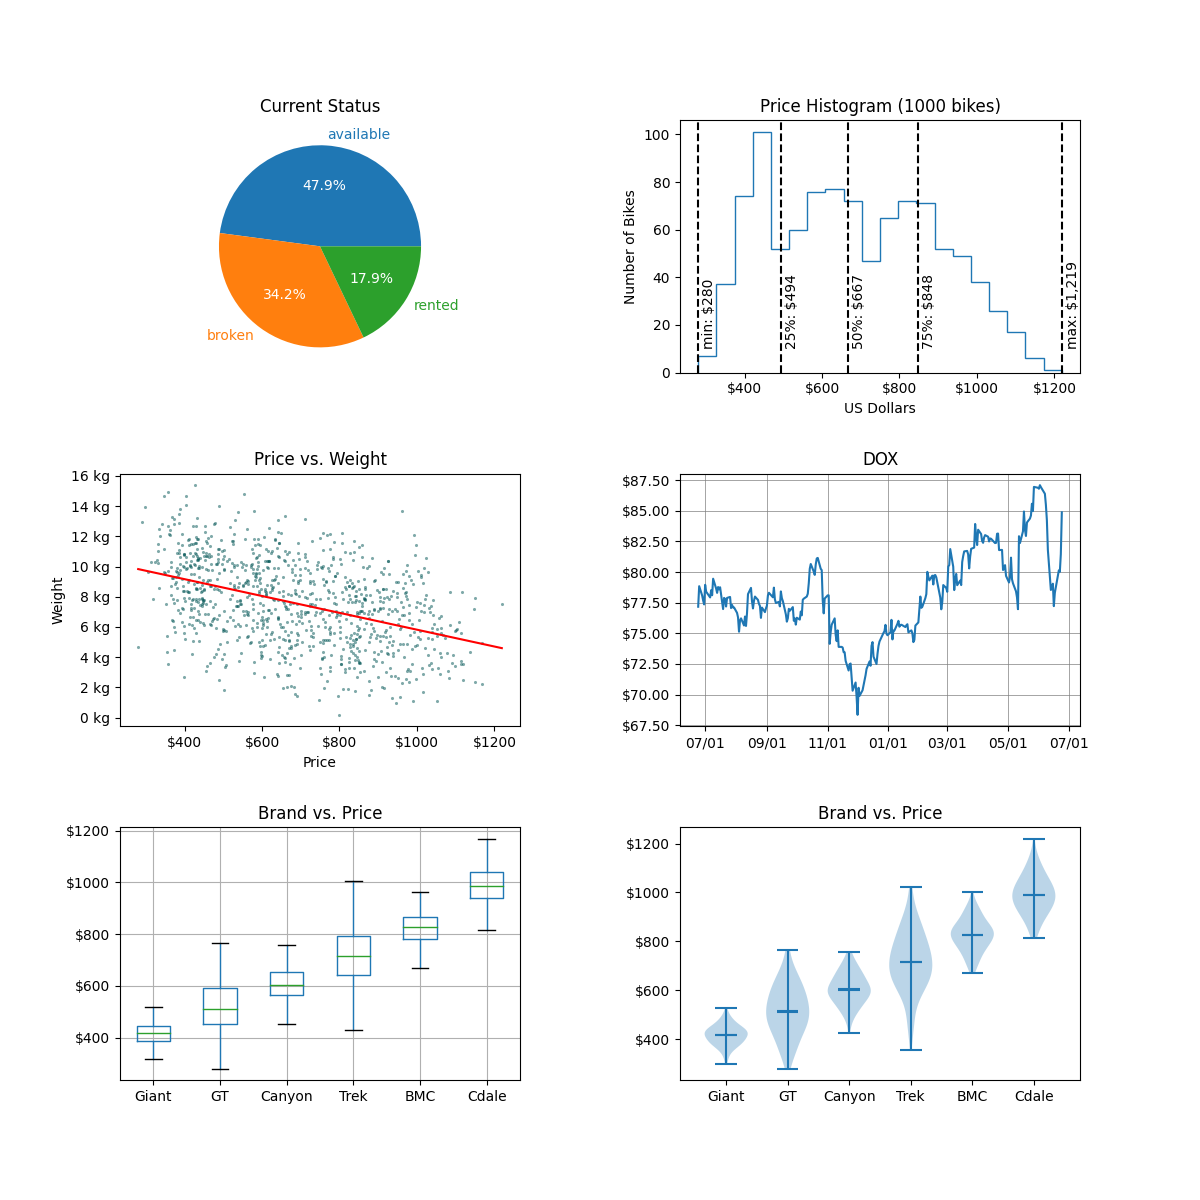
\includegraphics[width=\textwidth]{target.png}

Your score will be based upon how well your code generates a plot that matches this.

Your code should assume nothing about the data except the names of the columns.   That is, don't hard code any other assumptions about the data in your program.

We have not covered linear regression yet, so here is some code you can use.  Assuming that you have loaded the \texttt{bikes.csv} file into a pandas dataframe called \texttt{df}, this code will give you the slope and y-intercept of the red line in the scatter plot:

\begin{verbatim}
from sklearn.linear_model import LinearRegression

df = ...

# Get data as numpy arrays
X =  df['purchase_price'].values.reshape(-1, 1)
y = df['weight'].values.reshape(-1, 1)

# Do linear regression
reg = LinearRegression()
reg.fit(X, y)

# Get the parameters
slope = reg.coef_[0]
intercept = reg.intercept_
print(f"Slope: {slope}, Intercept: {intercept}")
\end{verbatim}


Do this work by yourself.   Stackoverflow is OK.   A hint from another student is OK.  Looking at another student's code is \emph{not} OK.

My solution is less than 80 lines of code.

\section{Derive a gradient}

\textit{1 point}

Let $f: R^3 \rightarrow R$ be given by

$$f(x, y,z) = y\sin(5x) + e^{yz} + \ln{z}$$

What is the gradient?

Answer: $\nabla f(x,y,z) =\begin{bmatrix} 5 y \cos{\left(5 x \right)},& z e^{y z} + \sin{\left(5 x \right)},& y e^{y z} + \frac{1}{z} \end{bmatrix}$

(Feel free to use sympy  if your calculus is a little rusty. )

Add the solution here in the LaTeX document and build a pdf from it.

\section{What to turn in}

If your name is Fred Jones, you will turn in a zip file called  \texttt{HW02\_Jones\_Fred.zip} of a directory called  \texttt{HW02\_Jones\_Fred}.  It will contain:
\begin{itemize}
\item \texttt{bikes.csv}
\item \texttt{DOX.csv}
\item \texttt{make\_plots.py}
\item \texttt{plots.png}
\item \texttt{Assignment.pdf}
\end{itemize}

Be sure to format your python code with black before you submit it.

We will unzip the directory and run your code like this:
\begin{verbatim}
cd HW02_Jones_Fred
python3 make_plots.py
\end{verbatim}

\section{Criteria for success}

And then we will look at the generated \texttt{plots.png}.  If your code doesn't run, you will lose points.  If \texttt{plots.png} doesn't look basically like \texttt{target.png}, you will lose points.

For the gradient,  the vector should be the correct length.  Each component should be correct.

\section{Extra help}

Here is a good video tutorial on Matplotlib:
\url{https://youtu.be/UO98lJQ3QGI}

Want to get ahead?  Web scraping is next:
\url{https://youtu.be/tb8gHvYlCFs}

\end{document}
